\documentclass[12pt]{article}
\usepackage{amsmath}
\usepackage{geometry}
\usepackage{booktabs}
\usepackage{enumerate}
\usepackage{amssymb}
\usepackage{graphicx}
\usepackage{subfigure}
\usepackage{upgreek}
\usepackage{multirow}
\usepackage{indentfirst}
\usepackage{color}
\usepackage{bm}
\usepackage{float}
\usepackage{caption}
\usepackage{amstext}
\usepackage{array}
\usepackage{enumerate}
\usepackage{subfigure}
\usepackage{listings}
\usepackage{xcolor}
\geometry{a4paper,left=2cm,right=2cm,top=2cm,bottom=2cm}
\thispagestyle{empty}
\lstset{
	language=Matlab, numbers=left, tabsize=4,
	framexleftmargin=1.5mm, frame=leftline,
	keywordstyle=\color{blue}\bfseries,
	identifierstyle=\bf, breaklines=true, 
	basicstyle=\normalsize,rulecolor=\color{brown}, 
	numberstyle=\color[RGB]{20,20,20}
}

\newcommand{\nullspacebig}{~\\[12pt]}
\newcommand{\nullspacesmall}{~\\[1pt]}
\newcommand{\nullspacemid}{~\\[80pt]}

\begin{document}
    \vspace{10cm}
    \begin{center}
        \rule{15cm}{0.01cm}
        \\\LARGE{
            UM-SJTU Joint Institute
            \\Vv285 / MATH285
          }
        \\\rule{15cm}{0.01cm}
        \\\vspace{6cm}
        \begin{Huge}
            1$^{st}$
        \end{Huge}
        \begin{Huge}
            \\\sc{UM-JI Integration Bee}
        \end{Huge}
    \end{center}
    \begin{figure}[H]
        \center
        
\includegraphics[width = 0.8\linewidth]{Figure/Logo.png}
    \end{figure}
    \vfill
    \flushleft
    \begin{center}
        \sc{Date: 3 July 2021}
    \end{center}

\setlength{\parindent}{1em}
\newpage
\thispagestyle{empty}
\setcounter{page}{1}

\section{Introduction}
\par \textbf{Integration Matters for Engineers!} While in Vv285(MATH285) we will discuss a lot about theoretical aspects of integration, the ability to evaluate concrete 
integrals is still indispensable. 

\par First, evaluation of concrete integrals is essential for doing hard analysis. Second, in higher level courses like VE215, VE203, VE216 and so on, calculation of integrals is 
common. Above all, this may help students prepare for exams of MATH285, since it is likely to contain more calculations than those in Vv186.

\par We would like to hold the first JI integration competition several days before Midterm 2. The integrals in the competition will mostly be on multi-variable or 
vector-valued functions, which are just what students will study before Midterm 2. Thus, the activity may help them review and solidify the knowledge they need for 
the exam.

\section{Objectives}
\begin{itemize}
    \item Help students get familiar with the procedure of solving problems related to course material.
    \item The idea came from MIT Integration Bee.  We have some students who are interested in it when we mentioned this back at Vv186.
\end{itemize}

\begin{figure}[H]
	\centering
	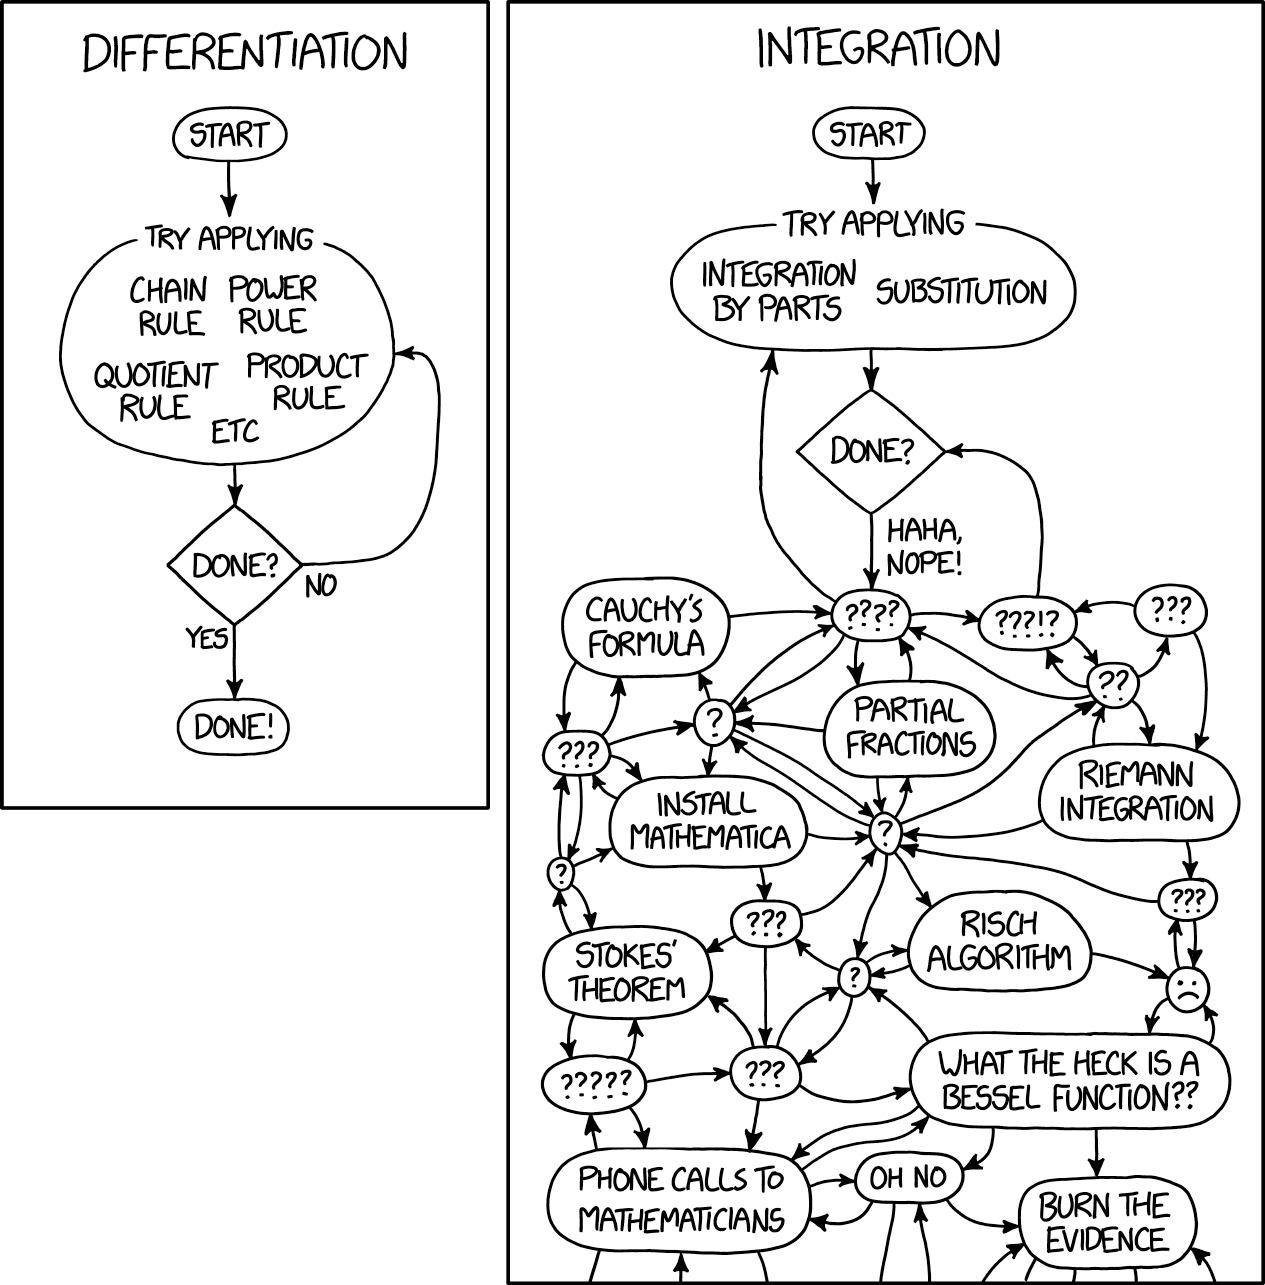
\includegraphics[width=0.7\linewidth]{Figure/pic1.png}
    \caption*{Integration is \textbf{HARD}!\protect\footnotemark}
\end{figure}

\footnotetext{https://xkcd.com/2117/}


\newpage


\section{Procedure}
\begin{itemize}
    \item To take part in the competition, every student will need to form a \textbf{group} for signing up.
    \item You can choose your teammates! Every group will have a maximum of \textbf{3 students}.
    \item We will design a problem sheet, which includes \textbf{15 problems}.
    \item Every group will have \textbf{60 minutes} to complete your work.
    \item The result will \textbf{only} depend on your answer, no procedure marks will be given.
    \item Every group can decide how to arrange their work. For example, one team can work on every question together and move on to the next problem together, 
    or each group member completes different problems by individuals.
\end{itemize}

\section{Regulation}
\par This is just a fun activity, but still please take it seriously. We don't want to see some cheater to win this activity! So only 
pencil and paper are allowed when you do your calculation. If one just plug in the function into, let's say Mathematica or Integral Calculator, then what's the point?
\begin{flushright}
    (p.s. If you want to bring a calculator, it's OK. But it is not so helpful anyway.)
\end{flushright}
\section{Rank}
\par The rank will \emph{only} depend on the score your group gets. Every question will have its points depending on how hard it is.
\par Additionally, if some groups' points are the same, \emph{we will hold an extra battle on the black board!}

\section{Prize}
\par \textbf{SECRET!} 
\par But we can make sure that everyone who attend this competition will get something!

\end{document}
